\section{Exercice 5}
\begin{enumerate}
  \item
        \q{On dispose d'une image en couleur (}\il{koala.jpg}\q{), on souhaite
          récupérer les pixels rouges dans un tableau et visualiser ce tableau
          en niveau de gris.}\\
        Question non traitée (par flemme...)

  \item
        \q{Appliquer le flitre ci-dessus à cette image et visualiser ces deux
          images côte à côte.}

        \bigskip

        Je définis les matrices des filtres suivantes :

        \bigskip

        \codeFromFile{section-02/q2-1.py}

        Puis je code la fonction \il{filtre}. Je n'afficherai le résultat qu'à la
        question suivante.
        \newpage
        \codeFromFile{section-02/q2-2.py}


  \item
        \q{Appliquer le flitre gaussien à cette même image.}

        \codeFromFile{section-02/q3-1.py}
        Ce qui donne, de gauche à droite : sans flitre, avec le flitre normal,
        avec le flitre gaussien :
\end{enumerate}

\begin{center}
  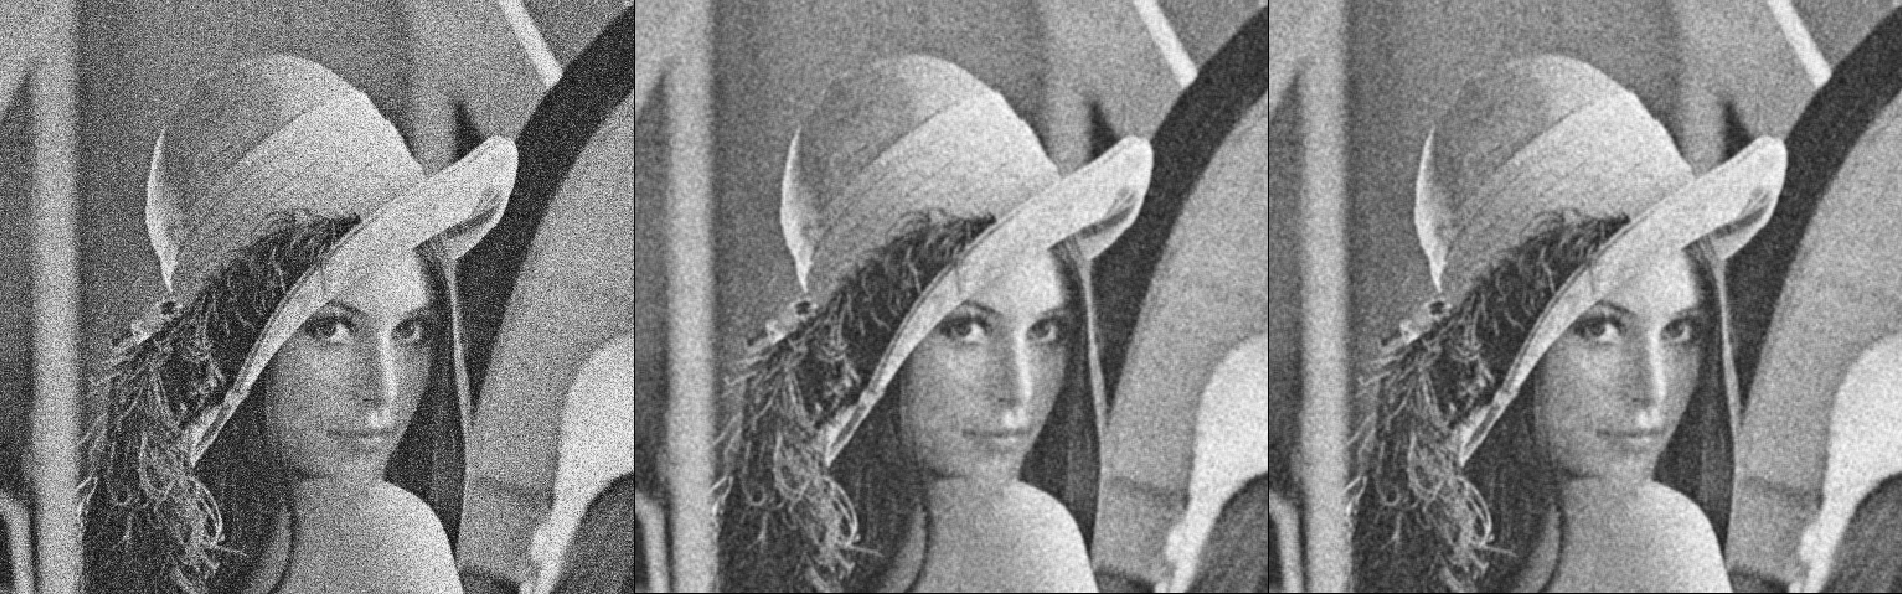
\includegraphics[scale=0.33]{section-02/q3-2.png}
\end{center}
